\documentclass[tikz,border=8pt]{standalone}
\usepackage{amsmath}\usepackage{pgfplots}\pgfplotsset{compat=1.18}
\definecolor{ink}{HTML}{21352F}\definecolor{teal}{HTML}{087F7B}\definecolor{gold}{HTML}{C58B2A}\definecolor{rose}{HTML}{B65A62}
\begin{document}
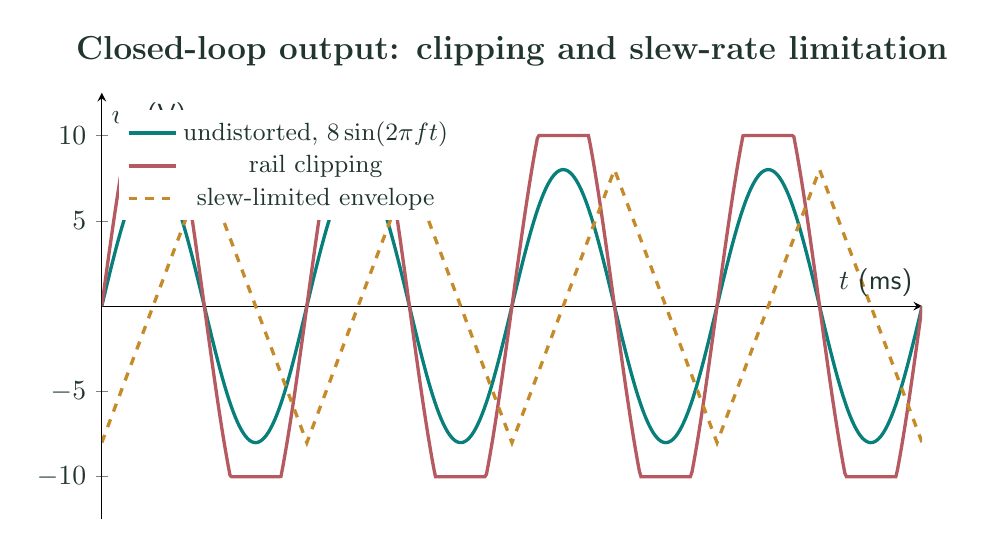
\begin{tikzpicture}[font=\sffamily,text=ink]
\begin{axis}[width=12cm,height=7cm,xmin=0,xmax=4,ymin=-12.5,ymax=12.5,axis lines=middle,xlabel={$t$ (ms)},ylabel={$v_o$ (V)},xtick=\empty,title={Closed-loop output: clipping and slew-rate limitation},title style={font=\bfseries\large},legend style={draw=none,at={(.02,.96)},anchor=north west,font=\small}]
 \addplot[teal,very thick,domain=0:4,samples=400] {8*sin(deg(2*pi*x))};\addlegendentry{undistorted, $8\sin(2\pi ft)$}
 \addplot[rose,very thick,domain=0:4,samples=500] {max(-10,min(10,14*sin(deg(2*pi*x))))};\addlegendentry{rail clipping}
 \addplot[gold,dashed,very thick] coordinates {(0,-8)(.5,8)(1,-8)(1.5,8)(2,-8)(2.5,8)(3,-8)(3.5,8)(4,-8)};\addlegendentry{slew-limited envelope}
\end{axis}
\end{tikzpicture}
\end{document}
